\documentclass[aspectratio=169,10pt]{beamer}

\usepackage[UTF8,fontset=fandol]{ctex}
\usepackage{fontspec}
\usepackage{graphicx}
\usepackage{booktabs}
\usepackage{array}
\usepackage{tikz}
\usepackage{amsmath,amssymb}
\usepackage{tabularx}
\usepackage{colortbl}
\usepackage{listings}
\usepackage{multirow}
\usetikzlibrary{arrows.meta,positioning,shapes.geometric,calc,fit,backgrounds}

\lstset{
  basicstyle=\ttfamily\scriptsize,
  keywordstyle=\color{Blue}\bfseries,
  commentstyle=\color{Muted}\itshape,
  stringstyle=\color{Teal},
  backgroundcolor=\color{Panel},
  frame=single,
  rulecolor=\color{Line},
  breaklines=true,
  showstringspaces=false,
  tabsize=4,
  language=Python,
}

\renewcommand{\sfdefault}{lmss}
\renewcommand{\familydefault}{\sfdefault}

% ──────────────────────────────────────────────
% Color Palette
% ──────────────────────────────────────────────
\definecolor{DeepNavy}{HTML}{172033}
\definecolor{Ink}{HTML}{273142}
\definecolor{Muted}{HTML}{667085}
\definecolor{SoftBlue}{HTML}{EAF2FF}
\definecolor{Blue}{HTML}{2F6FED}
\definecolor{Teal}{HTML}{00A6A6}
\definecolor{Orange}{HTML}{F59E0B}
\definecolor{Red}{HTML}{D64545}
\definecolor{Green}{HTML}{1F9D55}
\definecolor{Panel}{HTML}{F6F8FB}
\definecolor{Line}{HTML}{D8DEE9}
\definecolor{BoxBlue}{HTML}{D6E4FF}
\definecolor{BoxGreen}{HTML}{D1FAE5}
\definecolor{BoxOrange}{HTML}{FEF3C7}

% ──────────────────────────────────────────────
% Beamer Theme
% ──────────────────────────────────────────────
\setbeamercolor{normal text}{fg=Ink,bg=white}
\setbeamercolor{frametitle}{fg=DeepNavy,bg=white}
\setbeamercolor{title}{fg=DeepNavy}
\setbeamercolor{subtitle}{fg=Muted}
\setbeamercolor{block title}{fg=DeepNavy,bg=Panel}
\setbeamercolor{block body}{fg=Ink,bg=Panel}
\setbeamerfont{frametitle}{size=\Large,series=\bfseries}
\setbeamerfont{title}{size=\LARGE,series=\bfseries}
\setbeamerfont{subtitle}{size=\large}
\setbeamertemplate{navigation symbols}{}
\setbeamertemplate{itemize item}{\color{Blue}\small$\blacktriangleright$}
\setbeamertemplate{itemize subitem}{\color{Teal}\scriptsize$\bullet$}
\setbeamertemplate{enumerate item}{\color{Blue}\insertenumlabel.}
\setbeamertemplate{blocks}[rounded][shadow=false]

% Frametitle
\setbeamertemplate{frametitle}{
  \vspace{0.10cm}
  \begin{tikzpicture}[remember picture,overlay]
    \node[anchor=north east] at ($(current page.north east)+(-0.50cm,-0.18cm)$)
      {
\includegraphics[height=0.80cm]{figures/Sustech.png}};
  \end{tikzpicture}
  \begin{minipage}[t]{0.76\linewidth}
    \insertframetitle
  \end{minipage}
  \vspace{0.02cm}
  \par\textcolor{Line}{\rule{\linewidth}{0.65pt}}
}

% Footline
\setbeamertemplate{footline}{
  \leavevmode
  \hbox{
    \begin{beamercolorbox}[wd=.70\paperwidth,ht=2.6ex,dp=1.1ex,leftskip=0.55cm]{author in head/foot}
      \scriptsize\textcolor{Muted}{Reproducing Grounding DINO | CS308 Computer Vision | SUSTech}
    \end{beamercolorbox}
    \begin{beamercolorbox}[wd=.30\paperwidth,ht=2.6ex,dp=1.1ex,rightskip=0.55cm plus1fil]{date in head/foot}
      \scriptsize\hfill\textcolor{Muted}{\insertframenumber/\inserttotalframenumber}
    \end{beamercolorbox}
  }
}

% ──────────────────────────────────────────────
% Custom Commands
% ──────────────────────────────────────────────
\newcommand{\metric}[3]{%
  \begin{tikzpicture}
    \node[rounded corners=4pt, fill=#1!10, draw=#1!55, minimum width=2.2cm, minimum height=1.0cm, align=center] {
      {\Large\bfseries #2}\\[-1pt]{\scriptsize #3}
    };
  \end{tikzpicture}%
}
\newcommand{\smallnote}[1]{{\scriptsize\textcolor{Muted}{#1}}}

% ─ Style for TikZ flow nodes
\tikzset{
  flowbox/.style={
    rectangle, rounded corners=3pt, draw=Blue!60, fill=BoxBlue,
    text width=2.2cm, align=center, font=\scriptsize, minimum height=0.9cm
  },
  flowarrow/.style={-{Stealth}, Blue!60, thick},
  tokenok/.style={rectangle, rounded corners=2pt, draw=Green!60, fill=BoxGreen, font=\tiny, minimum width=1.6cm, minimum height=0.6cm, align=center},
  tokenbad/.style={rectangle, rounded corners=2pt, draw=Red!50, fill=Red!5, font=\tiny, minimum width=1.6cm, minimum height=0.6cm, align=center},
  tokensep/.style={rectangle, rounded corners=2pt, draw=Blue!60, fill=BoxBlue, font=\tiny, minimum width=0.6cm, minimum height=0.6cm},
}

% Placeholder slide macro
\newcommand{\placeholderslide}[1]{%
  \begin{frame}{#1}
    \centering
    \vspace{3cm}
    {\Large\textcolor{Muted}{[To be completed by other team members]}}
    \vspace{0.5cm}
    \smallnote{This slide is a placeholder — content to be added by the responsible team member.}
  \end{frame}
}

% ──────────────────────────────────────────────
% Title Info
% ──────────────────────────────────────────────
\title{复现 Grounding DINO：\\开放词汇目标检测与视觉定位}
\subtitle{Reproducing Grounding DINO: Open-Vocabulary Object Detection \\ and Visual Grounding on COCO 2017}
\author{苏思齐 (12310645) \quad 杨官宇涵 (12313614) \quad 莫丰源 (12311805)}
\institute{南方科技大学 (SUSTech)，深圳}
\date{\today}

\begin{document}

% ═══════════ Title Page ═══════════
{
\setbeamertemplate{footline}{}
\setbeamertemplate{frametitle}{}
\setbeamercolor{title}{fg=DeepNavy,bg=}
\setbeamercolor{subtitle}{fg=Muted,bg=}
\setbeamercolor{author}{fg=Ink,bg=}
\setbeamercolor{institute}{fg=Muted,bg=}
\setbeamercolor{date}{fg=Muted,bg=}
\setbeamerfont{title}{size=\Huge,series=\bfseries}
\setbeamerfont{subtitle}{size=\Large}
\setbeamerfont{author}{size=\footnotesize}
\setbeamerfont{institute}{size=\normalsize}
\usebackgroundtemplate{%
  \begin{tikzpicture}
    \node at (0.5\paperwidth,0.5\paperheight) {
\includegraphics[width=\paperwidth, height=\paperheight]{figures/background.png}};
    \fill[white,opacity=0.55] (0,0) rectangle (\paperwidth,\paperheight);
  \end{tikzpicture}%
}
\begin{frame}[plain]
  \vspace{0.6cm}
  \titlepage
  \vspace{-0.8cm}
  \begin{flushright}
    
\includegraphics[height=1.25cm]{figures/Sustech.png}\hspace{0.4cm}
  \end{flushright}
\end{frame}
}

% ═══════════ Outline ═══════════
\begin{frame}{提纲 (Outline)}
  \tableofcontents[subsectionstyle=show]
\end{frame}

% ═══════════ §1 Introduction (placeholder) ═══════════
\section{Introduction}
\placeholderslide{1. Introduction}

% ═══════════ §2 Related Works (placeholder) ═══════════
\section{Related Works}
\placeholderslide{2. Related Works}

% ══════════════════════════════════════════════
\section{Method}
% ══════════════════════════════════════════════

% --- Slide: Architecture Overview (with paper figure placeholder) ---
\begin{frame}{3.1 Model Architecture}
  \begin{columns}[T]
    \column{0.42\textwidth}
    \begin{block}{Three Core Components}
      \footnotesize
      \begin{enumerate}\setlength{\itemsep}{5pt}
        \item \textbf{Swin Transformer} (Liu et al., 2021)
              \begin{itemize}\scriptsize
                \item 4-stage hierarchical features (stride 4/8/16/32)
                \item Shifted-window attention, 28M params
              \end{itemize}
        \item \textbf{BERT Encoder} (Devlin et al., 2019)
              \begin{itemize}\scriptsize
                \item bert-base-uncased: 12 layers, hidden=768
                \item Contextualized token embeddings ($L \le 256$)
              \end{itemize}
        \item \textbf{Deformable Fusion}
              \begin{itemize}\scriptsize
                \item 6 layers, 8 heads, 900 object queries
                \item Cross-modal: visual locations $\leftrightarrow$ text tokens
              \end{itemize}
      \end{enumerate}
    \end{block}

    \column{0.56\textwidth}
    \centering
    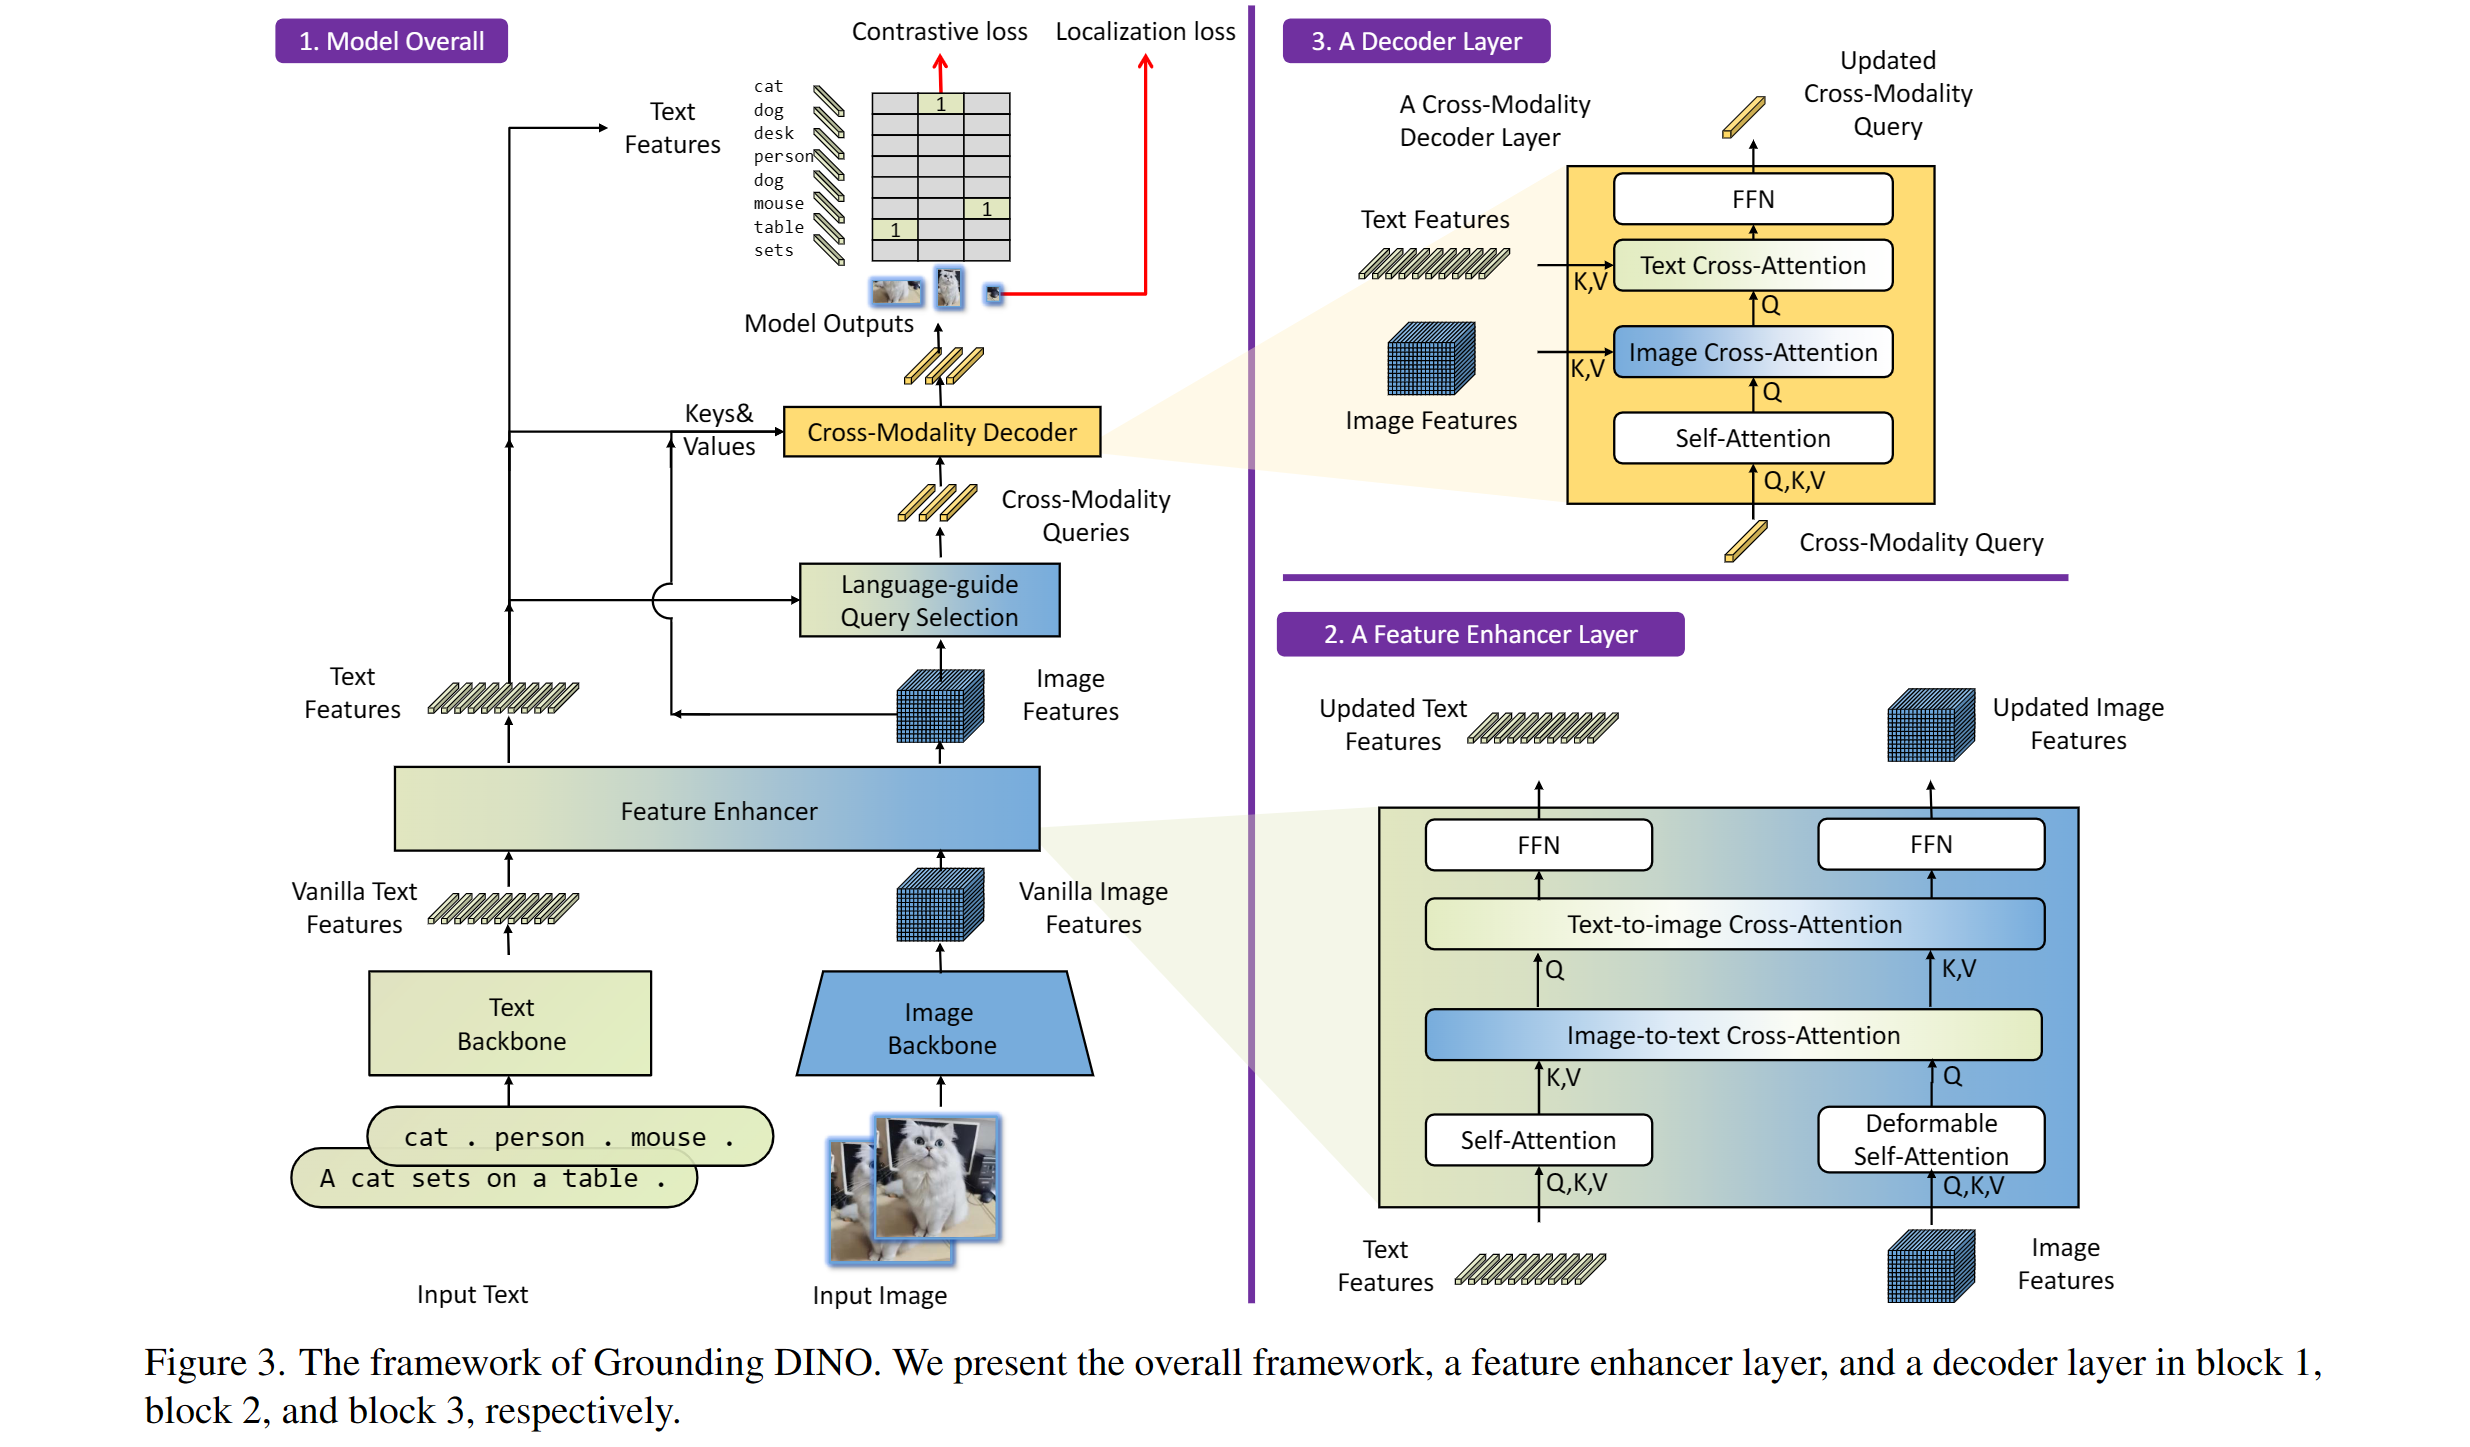
\includegraphics[width=0.95\linewidth]{figures/dinoarch.png}
    \vspace{0.1cm}

    \smallnote{Reproduction: zero-shot, fixed thresholds, single-scale, no fine-tuning.}
  \end{columns}
\end{frame}

% --- Slide: Inference Pipeline (TikZ flow diagram) ---
\begin{frame}{3.2 Inference Pipeline}
  \centering
  \vspace{0.3cm}

  % TikZ pipeline diagram
  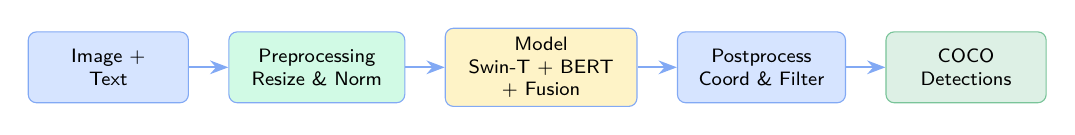
\begin{tikzpicture}[node distance=0.5cm]
    \node[flowbox, fill=BoxBlue, text width=1.8cm] (S1) {Image +\\Text};
    \node[flowbox, fill=BoxGreen, right=of S1, text width=2.0cm] (S2) {Preprocessing\\Resize \& Norm};
    \node[flowbox, fill=BoxOrange, right=of S2, text width=2.2cm] (S3) {Model\\Swin-T + BERT\\+ Fusion};
    \node[flowbox, fill=BoxBlue, right=of S3, text width=1.9cm] (S4) {Postprocess\\Coord \& Filter};
    \node[flowbox, fill=Green!15, draw=Green!60, right=of S4, text width=1.8cm] (S5) {COCO\\Detections};
    \draw[flowarrow] (S1) -- (S2);
    \draw[flowarrow] (S2) -- (S3);
    \draw[flowarrow] (S3) -- (S4);
    \draw[flowarrow] (S4) -- (S5);
  \end{tikzpicture}

  \vspace{0.4cm}
  \begin{columns}[T]
    \column{0.48\textwidth}
    \begin{block}{Key Parameters}
      \footnotesize
      \begin{itemize}\setlength{\itemsep}{2pt}
        \item Input: short side 800px, long side $\le$ 1333px
        \item Normalization: ImageNet mean/std
        \item Thresholds: box\_th=0.35, text\_th=0.25
        \item 900 queries $\times$ 256-dim features
      \end{itemize}
    \end{block}

    \column{0.48\textwidth}
    \begin{block}{Speed}
      \footnotesize
      \begin{itemize}\setlength{\itemsep}{2pt}
        \item $\sim$0.81 s/image on RTX 4060
        \item $\sim$68 min for full COCO val2017 (5,000 images)
        \item GPU memory peak: $\sim$3.2 GB
      \end{itemize}
    \end{block}
  \end{columns}
\end{frame}

% --- Slide: Prompt Design (TikZ tokenization comparison) ---
\begin{frame}{3.3 Prompt Design: Why Dot-Separated?}
  \centering
  \textbf{BERT WordPiece Tokenizer} — how the prompt is split into tokens:

  \vspace{0.2cm}
  % Dot-separated (GOOD)
  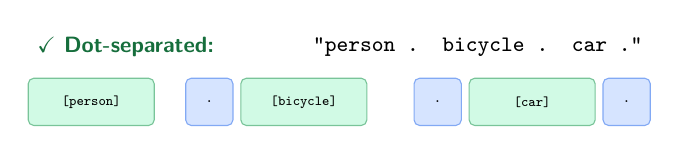
\begin{tikzpicture}
    \node[font=\footnotesize, anchor=west, text=Green!70!black] at (0,0) {\textbf{$\checkmark$ Dot-separated:}};
    \node[font=\footnotesize\ttfamily, anchor=west] at (3.5,0) {\texttt{"person . bicycle . car ."}};
    \node[tokenok, anchor=west] at (0,-0.7) {\texttt{[person]}};
    \node[tokensep, anchor=west] at (2.0,-0.7) {\texttt{.}};
    \node[tokenok, anchor=west] at (2.7,-0.7) {\texttt{[bicycle]}};
    \node[tokensep, anchor=west] at (4.9,-0.7) {\texttt{.}};
    \node[tokenok, anchor=west] at (5.6,-0.7) {\texttt{[car]}};
    \node[tokensep, anchor=west] at (7.3,-0.7) {\texttt{.}};
  \end{tikzpicture}

  \vspace{0.35cm}
  % Comma-separated (BAD)
  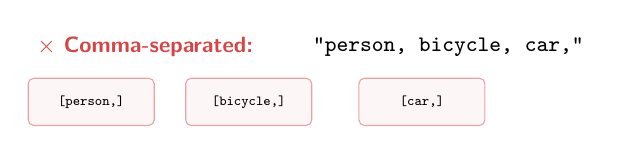
\begin{tikzpicture}
    \node[font=\footnotesize, anchor=west, text=Red] at (0,0) {\textbf{$\times$ Comma-separated:}};
    \node[font=\footnotesize\ttfamily, anchor=west] at (3.5,0) {\texttt{"person, bicycle, car,"}};
    \node[tokenbad, anchor=west] at (0,-0.7) {\texttt{[person,]}};
    \node[tokenbad, anchor=west] at (2.0,-0.7) {\texttt{[bicycle,]}};
    \node[tokenbad, anchor=west] at (4.2,-0.7) {\texttt{[car,]}};
  \end{tikzpicture}

  \vspace{0.3cm}
  \begin{columns}[T]
    \column{0.48\textwidth}
    \begin{block}{Why this matters}
      \footnotesize
      \begin{itemize}
        \item Period surrounded by spaces $\rightarrow$ independent separator token
        \item Comma merges with preceding word $\rightarrow$ ambiguous boundaries
        \item Non-dot formats cause \textbf{$\sim$62\% AP drop}
      \end{itemize}
    \end{block}

    \column{0.48\textwidth}
    \begin{block}{Phrase $\rightarrow$ Category}
      \footnotesize
      \begin{enumerate}\setlength{\itemsep}{2pt}
        \item \textbf{Exact match} (case-insensitive)
        \item \textbf{Substring match} (``dining'' $\rightarrow$ ``dining table'')
        \item \textbf{Alias match} (21-entry dict)
      \end{enumerate}
      $\sim$2--5\% phrases discarded when all layers fail.
    \end{block}
  \end{columns}
\end{frame}

% --- Slide: Software Architecture (compact) ---
\begin{frame}{3.4 Software Architecture}
  \begin{columns}[T]
    \column{0.50\textwidth}
    \begin{block}{5 Core Modules (1,826 LOC)}
      \footnotesize
      \renewcommand{\arraystretch}{1.1}
      \begin{tabular}{llr}
        \toprule
        \textbf{Module} & \textbf{Role} & \textbf{LOC} \\
        \midrule
        \texttt{models/} & Model wrapper & 182 \\
        \texttt{inference/predictor.py} & Inference API & 229 \\
        \texttt{inference/visualizer.py} & Draw boxes & 262 \\
        \texttt{engine/evaluator.py} & COCOeval & 368 \\
        \texttt{datasets/coco\_categories.py} & Prompt \& map & 269 \\
        \texttt{datasets/coco\_dataset.py} & Data utils & 188 \\
        \texttt{utils/box\_ops.py} & IoU, NMS & 115 \\
        \bottomrule
      \end{tabular}
    \end{block}

    \column{0.48\textwidth}
    \begin{block}{Design}
      \footnotesize
      \begin{itemize}\setlength{\itemsep}{3pt}
        \item \textbf{Config-driven}: OmegaConf YAML, CLI overrides
        \item \textbf{Modular}: 5 modules + 10 CLI scripts
        \item \textbf{Error-tolerant}: per-image try/except
      \end{itemize}
    \end{block}
    \vspace{0.1cm}
    \begin{block}{CLI Scripts (10)}
      \tiny
      inference.py | eval.py | run\_experiments.py

      download\_weights.py | download\_coco.py

      generate\_report\_highlights.py | generate\_visualizations.py

      train.py | setup\_env.sh | setup\_env.ps1
    \end{block}
  \end{columns}
\end{frame}

% ══════════════════════════════════════════════
\section{Experiments}
\subsection{4.1 Datasets}
% ══════════════════════════════════════════════

\begin{frame}{4.1 COCO 2017 Validation Set}
  \begin{columns}[T]
    \column{0.45\textwidth}
    \begin{block}{Overview (Lin et al., ECCV 2014)}
      \footnotesize
      \begin{itemize}\setlength{\itemsep}{4pt}
        \item \textbf{5,000 RGB images}, diverse real-world scenes
        \item \textbf{80 categories} (person, car, dog, chair, \ldots)
        \item \textbf{36,781 GT boxes} — avg $\sim$7.4 per image
        \item \textbf{Long-tail distribution}: ``person'' dominates; ``hair drier'' $<$100
      \end{itemize}
    \end{block}
    \vspace{0.1cm}
    \begin{block}{Splits}
      \footnotesize
      \renewcommand{\arraystretch}{1.1}
      \begin{tabular}{lcc}
        \toprule
        \textbf{Split} & \textbf{Images} & \textbf{Usage} \\
        \midrule
        train2017 & 118K & Fine-tuning \\
        \textbf{val2017} & \textbf{5,000} & \textbf{Evaluation} \\
        test2017 & 40K & Benchmark \\
        \bottomrule
      \end{tabular}
    \end{block}

    \column{0.53\textwidth}
    \centering
    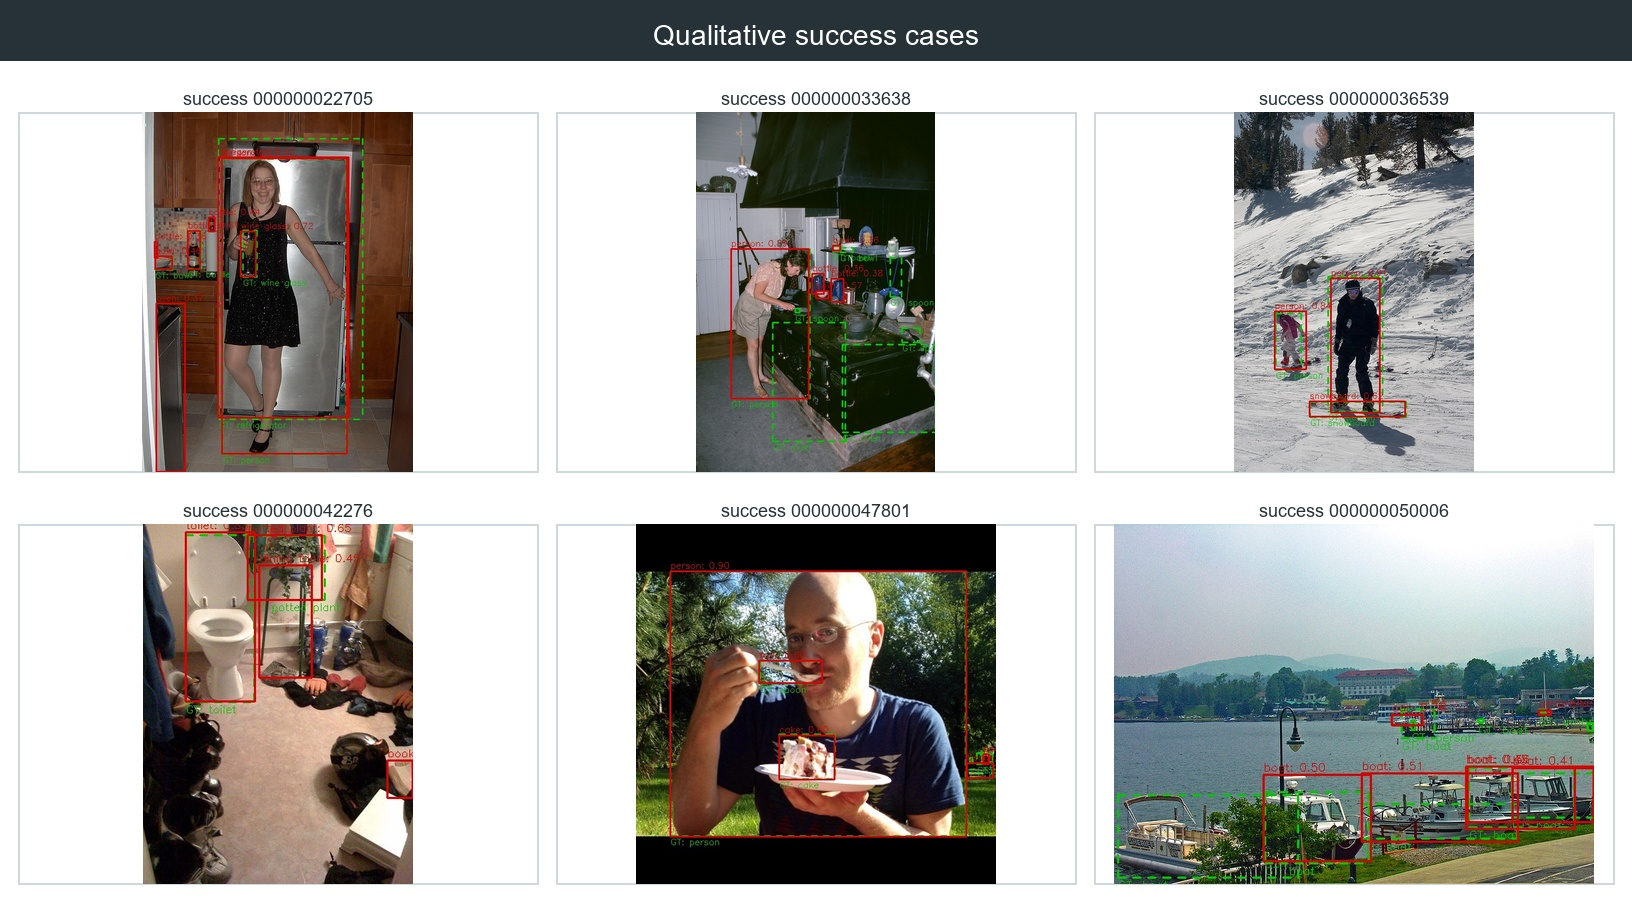
\includegraphics[width=0.95\linewidth]{figures/05_success_cases_grid.jpg}
    \vspace{0.1cm}
    \smallnote{Example COCO val2017 images with Grounding DINO zero-shot detections}
  \end{columns}
\end{frame}

% ─ Placeholders ─
\subsection{4.2 Implementation Details}
\placeholderslide{4.2 Implementation Details}
\subsection{4.3 Metrics}
\placeholderslide{4.3 Metrics}
\subsection{4.4 Experimental Design \& Results}
\placeholderslide{4.4 Experimental Design \& Results}

% ══════════════════════════════════════════════
\section{Conclusion}
% ══════════════════════════════════════════════

\begin{frame}{5. Conclusion}
  \vspace{-0.2cm}
  \begin{columns}[T]
    \column{0.55\textwidth}
    \begin{block}{Problem \& Approach}
      \footnotesize
      \textbf{Challenge}: Open-vocabulary object detection — detect arbitrary categories without per-category training data.

      \textbf{Method}: Reproduced Grounding DINO (Liu et al., ECCV 2024) with Swin-Tiny backbone, zero-shot on COCO 2017 val2017.

      \textbf{Setup}: Config-driven, dot-separated prompts, box\_th=0.35, single-scale, no fine-tuning.
    \end{block}

    \column{0.43\textwidth}
    \begin{block}{Key Findings}
      \footnotesize
      \begin{enumerate}\setlength{\itemsep}{2pt}
        \item Zero-shot detection is viable without task-specific training
        \item Threshold selection critically impacts precision-recall
        \item Dot-separated prompts are a functional requirement
        \item Small-object detection is the primary bottleneck
        \item Localization lags behind recognition
      \end{enumerate}
    \end{block}
  \end{columns}

  \vspace{0.15cm}
  \centering
  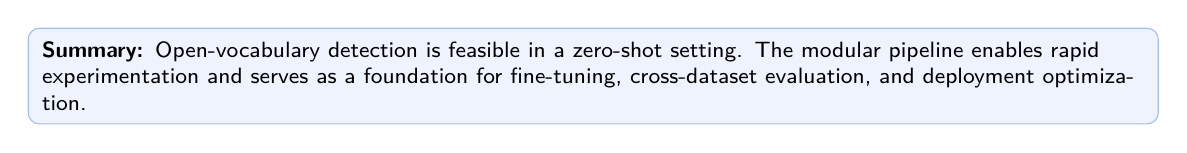
\begin{tikzpicture}
    \node[rounded corners=4pt, fill=Blue!8, draw=Blue!45, text width=14cm, inner sep=5pt, font=\footnotesize] {
      \textbf{Summary:} Open-vocabulary detection is feasible in a zero-shot setting.
      The modular pipeline enables rapid experimentation and serves as a foundation
      for fine-tuning, cross-dataset evaluation, and deployment optimization.
    };
  \end{tikzpicture}
\end{frame}

% ══════════════════════════════════════════════
\section{References}
% ══════════════════════════════════════════════

\begin{frame}{References}
  \footnotesize
  \renewcommand{\arraystretch}{1.4}
  \begin{enumerate}\setlength{\itemsep}{2pt}
    \item \textbf{Grounding DINO}: S. Liu et al., ``Grounding DINO: Marrying DINO with Grounded Pre-Training for Open-Set Object Detection,'' \textit{ECCV}, 2024.
    \item \textbf{DINO}: H. Zhang et al., ``DINO: DETR with Improved DeNoising Anchor Boxes for End-to-End Object Detection,'' \textit{ICLR}, 2023.
    \item \textbf{DETR}: N. Carion et al., ``End-to-End Object Detection with Transformers,'' \textit{ECCV}, 2020.
    \item \textbf{Deformable DETR}: X. Zhu et al., ``Deformable DETR: Deformable Transformers for End-to-End Object Detection,'' \textit{ICLR}, 2021.
    \item \textbf{Swin Transformer}: Z. Liu et al., ``Swin Transformer: Hierarchical Vision Transformer using Shifted Windows,'' \textit{ICCV}, 2021.
    \item \textbf{BERT}: J. Devlin et al., ``BERT: Pre-training of Deep Bidirectional Transformers for Language Understanding,'' \textit{NAACL}, 2019.
    \item \textbf{GLIP}: L. H. Li et al., ``Grounded Language-Image Pre-training,'' \textit{CVPR}, 2022.
    \item \textbf{OWL-ViT}: M. Minderer et al., ``Simple Open-Vocabulary Object Detection with Vision Transformers,'' \textit{ECCV}, 2022.
    \item \textbf{YOLO-World}: T. Cheng et al., ``YOLO-World: Real-Time Open-Vocabulary Object Detection,'' \textit{CVPR}, 2024.
    \item \textbf{COCO}: T.-Y. Lin et al., ``Microsoft COCO: Common Objects in Context,'' \textit{ECCV}, 2014.
    \item \textbf{CLIP}: A. Radford et al., ``Learning Transferable Visual Models From Natural Language Supervision,'' \textit{ICML}, 2021.
  \end{enumerate}
\end{frame}

% ══════════════════════════════════════════════
\section{Contributions}
% ══════════════════════════════════════════════

\begin{frame}{Contributions}
  \begin{columns}[T]
    \column{0.32\textwidth}
    \begin{block}{苏思齐 (12310645)}
      \scriptsize
      \begin{itemize}\setlength{\itemsep}{2pt}
        \item [To be completed]
        \item [To be completed]
        \item [To be completed]
      \end{itemize}
    \end{block}

    \column{0.36\textwidth}
    \begin{block}{杨官宇涵 (12313614)}
      \scriptsize
      \begin{itemize}\setlength{\itemsep}{2pt}
        \item 整体项目设计与实现
        \item 全部 Python 模块与 CLI 脚本编写
        \item 完整 COCO 评估与消融实验执行
        \item 报告撰写
      \end{itemize}
    \end{block}

    \column{0.30\textwidth}
    \begin{block}{莫丰源 (12311805)}
      \scriptsize
      \begin{itemize}\setlength{\itemsep}{2pt}
        \item [To be completed]
        \item [To be completed]
        \item [To be completed]
      \end{itemize}
    \end{block}
  \end{columns}

  \vspace{0.5cm}
  \centering
  \Large\textbf{Thank You!} \quad \normalsize Q \& A
\end{frame}

\end{document}
